\documentclass[journal,10pt]{IEEEtran}

\usepackage[T1]{fontenc}
\usepackage[utf8]{inputenc}
\usepackage{lmodern}
\usepackage{microtype}
\usepackage{amsmath,amssymb,mathtools}
\usepackage{booktabs}
\usepackage{multirow}
\usepackage{array}
\usepackage{graphicx}
\usepackage{siunitx}
\usepackage{algorithm2e}
\usepackage{tikz}
\usetikzlibrary{arrows.meta,positioning,fit,shapes.geometric}
\usepackage{enumitem}
\usepackage{xcolor}
\usepackage{hyperref}
\usepackage[capitalise,noabbrev]{cleveref}

\hypersetup{
  colorlinks=true,
  linkcolor=black,
  citecolor=black,
  urlcolor=black,
  pdfauthor={Othmane Hassani},
  pdftitle={Robust ML-Assisted Optimal Execution in Limit Order Books},
  pdfsubject={Controlled and reproducible study of prediction, control, robustness, and systems trade-offs in optimal execution},
  pdfkeywords={optimal execution, limit order book, causal prediction, model predictive control, reinforcement learning, robustness, reproducibility}
}

\sisetup{detect-all,round-mode=places,round-precision=3}
\graphicspath{{figures/}}
\newcommand{\bps}{\ensuremath{\,\mathrm{bps}}}
\newcommand{\E}{\mathbb{E}}
\newcommand{\R}{\mathbb{R}}
\newcommand{\1}{\mathbf{1}}
\newcommand{\clip}{\operatorname{clip}}
\newcommand{\CVaR}{\operatorname{CVaR}}
\newcommand{\IS}{\operatorname{IS}}

\title{Robust ML-Assisted Optimal Execution in Limit Order Books:\\
Causal Microstructure Forecasting, Model Predictive Control, and Low-Latency Systems Evaluation}

\author{Othmane~Hassani% <-this % stops a space
\thanks{O. Hassani is with ESILV Graduate School of Engineering, De Vinci Higher Education, Paris-La D\'efense, France. Source and artifacts: \url{https://github.com/000zer000/robust-ml-optimal-execution}.}}

\begin{document}
\maketitle

\begin{abstract}
Optimal execution couples predictive signal, market mechanics, queue uncertainty, transaction costs, latency, and computation. We present a reproducible C++/Python research system that asks whether an improved causal limit-order-book forecast survives the downstream optimization map and improves execution. The design combines exact integer-arithmetic matching and accounting, explicit aggregate-L2 queue scenarios, strong classical baselines, matched non-ML and ML-assisted model-predictive controllers (MPC), a compact Conv1D--LSTM, imitation learning with dataset aggregation, categorical proximal policy optimization (PPO), registered stress tests, paired block-bootstrap inference, and end-to-end CPU/GPU measurement. All strategy findings are registered controlled-simulator evidence, not historical-market backtests; systems findings are direct measurements on identified hardware.

The experiments reveal non-monotone proxy relationships. Calibration can improve log loss yet weaken controller response, and a perfect intermediate-event oracle can worsen implementation shortfall. An imitation student achieves exact controlled-holdout agreement but loses fidelity under distribution shift; PPO does not dominate strong deterministic heuristics. Across 43 stress conditions, the lowest-cost strategy changes in 16 of 42 non-central regimes. Of 129 paired contrasts, 85 confidence intervals cross zero, and 22 of 43 point winners have less than 80\% bootstrap probability of remaining best. A profile-guided C++ optimization reaches 17.316 million operations/s in the measured four-thread workload. On a Tesla T4, transfer-inclusive GPU inference is slower for every registered batch-one workload; the temporal model becomes GPU-favorable at batch 256 with a 1.704$\times$ speedup. The evidence supports a methodological conclusion: predictive accuracy, decision value, policy complexity, robustness, and hardware acceleration should be evaluated through one causal execution-and-accounting pipeline rather than optimized as independent proxies.
\end{abstract}

\begin{IEEEkeywords}
optimal execution, limit order book, market microstructure, model predictive control, causal machine learning, imitation learning, reinforcement learning, robustness, reproducibility.
\end{IEEEkeywords}

\section{Introduction}
\label{sec:intro}
Electronic execution converts a parent trading instruction into a sequence of child orders while attempting to control explicit transaction costs, market impact, adverse price movement, timing risk, and non-completion risk. The classical optimal-execution literature formalizes this trade-off through dynamic control and market-impact models \cite{BertsimasLo1998,AlmgrenChriss2001,ObizhaevaWang2013,AlfonsiFruthSchied2010,Gatheral2010}. In modern limit-order-book (LOB) markets, however, the execution problem is more granular. The controller observes finite displayed depth, queue state only imperfectly, rapidly evolving order flow, fee and latency effects, and an action space containing both liquidity-providing and liquidity-taking decisions. The relevant state is therefore partly predictive and partly mechanical.

Machine learning offers a natural way to compress short-horizon order-flow information into forecasts. DeepLOB and subsequent work demonstrate that nonlinear models can extract predictive structure from LOB states and order-flow imbalance \cite{ZhangZohrenRoberts2019,SirignanoCont2019,KolmTurielWestray2023,BriolaBartolucciAste2025}. Yet forecasting performance and execution value are not equivalent objectives. A model may reduce log loss without changing the optimizer's action; a poorly calibrated change near a decision boundary may alter an action more than a globally better predictor; and a target that is statistically learnable may be only indirectly related to implementation shortfall. This distinction is closely related to the predict-then-optimize and decision-focused learning literature \cite{ElmachtoubGrigas2022,DontiAmosKolter2017,WilderDilkinaTambe2019}.

A second complication is that policy sophistication is not synonymous with robustness. Reinforcement-learning (RL) execution systems can adapt to state-dependent environments \cite{NevmyvakaFengKearns2006,ZhangDuanChen2023,WangGaoLi2026,CheriditoWeiss2026}, but simulator misspecification, reward design, distribution shift, and random-seed sensitivity can dominate apparent improvements. A third complication is computational: inference and control latency become endogenous execution costs. A GPU kernel may be fast in isolation while host-device transfers make the complete decision path slower than CPU inference.

This work treats these issues as a single systems-and-decision problem. Rather than optimizing a forecasting benchmark, an RL score, or a microbenchmark independently, it builds a reproducible pipeline from market events to execution accounting and asks how each layer changes downstream decisions. The research system is designed around five principles: exact market-state semantics, causal information timing, matched controller comparisons, stress testing under model uncertainty, and measurement-driven performance engineering.

\subsection{Research Questions}
The study is organized around the following questions.
\begin{enumerate}[leftmargin=*,label=\textbf{RQ\arabic*:}]
    \item Can short-horizon causal microstructure forecasts alter execution decisions when injected into a queue-aware finite-horizon controller without changing the controller's optimizer or mechanical assumptions?
    \item Does improved predictive quality translate monotonically into improved decision quality or implementation shortfall?
    \item Can a compact learned policy reproduce an optimizer sufficiently well to reduce inference latency, and how does imitation degrade under covariate shift?
    \item Does an RL execution policy provide robust cost improvements over strong deterministic baselines across multiple seeds and stress regimes?
    \item How stable are strategy rankings under paired uncertainty analysis and multiplicity control?
    \item Which parts of the execution stack benefit from CPU parallelism, compiled inference, or GPU acceleration once end-to-end transfer costs are included?
\end{enumerate}

\subsection{Contributions}
The primary contributions are:
\begin{itemize}[leftmargin=*]
    \item an exact, deterministic C++ market, queue-scenario, and execution-accounting core that gives classical schedules, MPC, imitation, and RL policies one mechanical comparison path;
    \item a matched forecast-to-control experiment combining a causal 20-feature model ladder with neutral, shuffled, stale, uncalibrated, perfect-event-oracle, and zero-weight ablations, isolating when predictive improvement does or does not create decision value;
    \item an integrated sequential-policy evaluation spanning exact-teacher imitation, validation-triggered DAgger, conservative OOD fallback, multi-seed categorical PPO, 43 registered stress conditions, and dependence-aware ranking inference;
    \item a reproducible systems study that measures correctness-preserving C++ optimization, multithread scaling, the Python/C++ boundary, compiled inference, and transfer-inclusive Tesla T4 timing on the complete registered workloads.
\end{itemize}

\section{Related Work}
\label{sec:related}
\subsection{Optimal Execution and Market Impact}
The canonical execution problem trades immediacy against market impact and price risk. Bertsimas and Lo formulate execution as stochastic control \cite{BertsimasLo1998}; Almgren and Chriss derive the widely used mean--variance frontier between expected impact cost and execution risk \cite{AlmgrenChriss2001}. Subsequent models enrich impact dynamics and order-book structure, including transient resilience \cite{ObizhaevaWang2013}, general LOB shape functions \cite{AlfonsiFruthSchied2010}, no-dynamic-arbitrage restrictions on impact kernels \cite{Gatheral2010}, and adaptive execution \cite{LorenzAlmgren2011}. Limit and market order control introduces an additional fill-versus-adverse-selection trade-off \cite{CarteaJaimungal2015,GueantLehalleFernandezTapia2012}.

The present system uses these works as structural guidance rather than attempting to reproduce a single closed-form model. In particular, execution costs are computed from actual simulated fills and fees, while the controller includes explicit inventory and terminal penalties. This separation keeps accounting exact even when control heuristics are approximate.

\subsection{Limit-Order-Book Dynamics and Queue Uncertainty}
LOB state evolves through order arrivals, cancellations, modifications, and trades. Markovian and queue-reactive models show how state-dependent intensities and queue dynamics affect short-horizon price behavior \cite{ContStoikovTalreja2010,ContDeLarrard2013,HuangLehalleRosenbaum2015}. Order-flow imbalance and book events are strongly connected to near-term price impact \cite{ContKukanovStoikov2014,BouchaudFarmerLillo2009}. Gould et al. provide a broad review of the empirical and modeling literature \cite{GouldPorterWilliamsMcDonaldFennHowison2013}.

Aggregate L2 data creates a specific identification problem: a reduction in displayed size at a price cannot generally be decomposed uniquely into cancellations ahead of a child order, cancellations behind it, or hidden execution. The system therefore treats queue position as a scenario variable. The three queue models in \cref{sec:queue} deliberately bracket this uncertainty rather than turning aggregate depth into an unjustified exact fill probability.

\subsection{Machine Learning for LOB Forecasting}
DeepLOB combines convolutional and recurrent processing for LOB forecasting \cite{ZhangZohrenRoberts2019}; Sirignano and Cont study common price-formation structure across instruments \cite{SirignanoCont2019}; and deep order-flow imbalance work demonstrates cross-horizon predictive content \cite{KolmTurielWestray2023}. Recent surveys emphasize that target definition, normalization, leakage control, and horizon selection can be as important as architecture \cite{BriolaBartolucciAste2025}. Calibration is also critical when predicted probabilities are consumed by downstream optimizers \cite{GuoPleissSunWeinberger2017}. The gap addressed here is therefore not another forecasting leaderboard: it is an end-to-end, matched test of the path from forecast score to controller action, realized execution cost, stress robustness, and compute latency.

This work uses a deliberately compact temporal model and a strong simple-model ladder. The objective is not architecture novelty. Instead, forecasting is treated as an intermediate input whose value is tested by the execution controller.

\subsection{Decision-Focused Prediction}
Predict-then-optimize research demonstrates that minimizing prediction error need not minimize downstream decision loss \cite{ElmachtoubGrigas2022}. Task-based and decision-focused methods explicitly differentiate or otherwise learn through optimization objectives \cite{DontiAmosKolter2017,WilderDilkinaTambe2019}. The experiments in this paper do not replace the execution optimizer with a differentiable surrogate; instead, they perform controlled ablations that reveal where the prediction-to-decision map becomes non-monotonic. This provides a diagnostic foundation for future decision-focused training.

\subsection{Imitation and Reinforcement Learning for Execution}
DAgger addresses covariate shift in behavior cloning by querying an expert on learner-visited states and aggregating corrective data \cite{RossGordonBagnell2011}. This mechanism is particularly relevant in execution because small action errors alter future inventory and market interaction, causing the state distribution to drift from the teacher's demonstration distribution.

RL has a longer history in execution, from early optimized trade-execution agents \cite{NevmyvakaFengKearns2006} to recent work on cross-environment generalization \cite{ZhangDuanChen2023}, continuous-time actor--critic methods \cite{WangGaoLi2026}, queue-reactive environments \cite{EspanaHafsiLilloVittori2025}, and joint market/limit-order policies \cite{CheriditoWeiss2026}. PPO provides a simple clipped policy-gradient objective with multiple minibatch epochs per on-policy sample \cite{SchulmanWolskiDhariwalRadfordKlimov2017}. The present experiments use one predeclared PPO family and report all registered seeds rather than selecting the best seed.

\subsection{Market Simulation, Robustness, and Reproducibility}
Simulation fidelity is central to any learning-based trading experiment. ABIDES provides an agent-based market simulation framework \cite{ByrdHybinetteBalch2019}; JAX-LOB demonstrates GPU-accelerated LOB simulation for large-scale RL \cite{FreyLiNagy2023}; realism metrics and benchmarking frameworks make simulator quality explicit \cite{VyetrenkoByrdPetosa2020,NagyFreyLi2025}; and recent work studies queue-reactive deep simulation and the simulation-to-reality gap \cite{BodorCarlier2025,NobleRosenbaumSouilmi2026}. The statistical layer of this project draws on block-bootstrap and multiple-testing ideas appropriate for dependent experiments \cite{PolitisRomano1994,White2000,RomanoWolf2005}. Reproducible configurations, seed reporting, compute disclosure, and deterministic regeneration follow the broader ML reproducibility principles summarized by Pineau et al. \cite{PineauVincentLamarreSinhaLariviere2021}.

\section{Problem Formulation}
\label{sec:problem}
Consider a parent order of size $Q>0$ submitted at decision time $t_0$, with side sign $s\in\{+1,-1\}$ for buy and sell, respectively. The benchmark price is the arrival mid or configured arrival benchmark $P_0$. A policy generates a sequence of child actions $a_k$ at decision times $t_k$ based on the causal state $x_k$. Fills are indexed by $i$ and have quantity $q_i$, execution price $P_i$, and explicit fee/rebate contribution $f_i$.

\subsection{Implementation Shortfall}
Let executed notional and benchmark notional be
\begin{align}
N_{\mathrm{exec}} &= \sum_i P_i q_i, \\
N_{\mathrm{bench}} &= P_0 Q,
\end{align}
with total fees $F=\sum_i f_i$. The signed implementation shortfall in quote units is
\begin{equation}
\IS = s\left(N_{\mathrm{exec}}-N_{\mathrm{bench}}\right)+F,
\label{eq:is}
\end{equation}
and the normalized shortfall is
\begin{equation}
\IS_{\mathrm{bps}}=10^4\frac{\IS}{N_{\mathrm{bench}}}.
\label{eq:is-bps}
\end{equation}
Positive values are worse execution; negative values represent price improvement relative to the arrival benchmark. The accounting layer computes \cref{eq:is} from fills rather than from controller estimates. Incomplete orders do not receive a misleading final shortfall; terminal completion is charged explicitly through the configured completion mechanism.

\subsection{State and Action Space}
A generic execution state is
\begin{equation}
x_k=(B_k, A_k, I_k, \tau_k, z_k, \ell_k, c_k),
\end{equation}
where $B_k$ and $A_k$ denote the observable bid/ask books, $I_k$ is remaining inventory, $\tau_k$ is time remaining, $z_k$ collects causal order-flow features, $\ell_k$ denotes latency state, and $c_k$ contains fee/impact parameters. Classical policies use a subset of this state; learned policies receive explicitly frozen feature vectors.

The finite execution action family contains no action, passive placement at bounded fractions of remaining inventory, and aggressive execution. The RL environment expands this into six discrete actions:
\begin{equation}
\mathcal{A}=\{\text{wait},P_{25},P_{50},A_{25},A_{50},A_{100}\}.
\label{eq:rl-actions}
\end{equation}
Action validation is centralized so that model, heuristic, and RL policies cannot bypass tick/lot, inventory, or terminal constraints.

\subsection{Execution Cost Decomposition}
For a child fill of fraction $\rho=q/Q$, the controlled environment uses a cost decomposition of the form
\begin{equation}
C_{\mathrm{fill}} = C_{\mathrm{price}} + \rho\left(C_{\mathrm{impact}} + C_{\mathrm{latency}} + C_{\mathrm{fee}} + C_{\mathrm{adverse}}\right),
\label{eq:fill-cost}
\end{equation}
where impact can scale as
\begin{equation}
C_{\mathrm{impact}} = \eta\left(\frac{q}{D}\right)^\gamma,
\end{equation}
Here $D$ is visible depth, $\eta$ is the impact coefficient, and the central controlled configuration sets $\gamma=2$. Inventory exposure is penalized quadratically,
\begin{equation}
C_{\mathrm{inv},k}=\lambda_I\left(\frac{I_k}{Q}\right)^2,
\label{eq:inventory-risk}
\end{equation}
with an explicit terminal charge for forced completion.

\section{Exact Market and Execution Infrastructure}
\label{sec:infrastructure}
\subsection{Canonical Event Representation}
The simulator uses exact integer arithmetic for the market-state quantities that define matching semantics. Price is represented as signed 64-bit ticks, quantity as unsigned 64-bit lots, and quote notional as signed integer quote atoms with rational tick and lot sizes. Timestamps are nanosecond-resolution integers accompanied by an explicit clock domain. This eliminates floating-point ambiguity from price-level identity and quantity conservation.

Deterministic event ordering uses the lexicographic key
\begin{equation}
K(e)=(t_e,\,s_e,\,u_e,\,g_e,\,i_e),
\label{eq:event-key}
\end{equation}
where $t_e$ is event time, $s_e$ canonical sequence, $u_e$ source subsequence, $g_e$ ingestion sequence, and $i_e$ internal event identifier. Canonical JSONL audit events are chained by SHA-256, allowing replay artifacts to be checked for accidental mutation.

\subsection{Matching Engine}
The C++ matching engine enforces price-time ordering at the modeled level, exact tick/lot validation, quantity conservation, deterministic child-order identifiers, and explicit order lifecycle state. Aggressive execution sweeps visible depth level by level; passive execution is delegated to the queue model and cannot fill before activation. The same accounting objects feed execution metrics, controller tests, and policy environments.

\subsection{Data Admission and Replay}
Historical/live ingestion is organized around immutable source manifests, clock metadata, symbol normalization, schema validation, and quarantine rules. Sequence gaps, malformed timestamps, impossible book states, and incomplete spans are rejected rather than silently interpolated. The controlled numerical experiments reported in this manuscript are generated by the validated deterministic simulation path; hardware measurements are empirical on the processors identified in \cref{sec:performance}. Keeping these evidence classes separate makes model-risk experiments reproducible while preserving a distinct external-feed replay path.

\subsection{Aggregate-L2 Queue Models}
\label{sec:queue}
At passive activation, a child order is placed behind all displayed same-price quantity. Subsequent increases at that level are placed behind the child. The ambiguous case is an unexplained reduction in displayed size. Three queue assumptions bracket the unknown position of cancellations:
\begin{enumerate}[leftmargin=*]
    \item \textbf{Optimistic:} unexplained displayed reductions are allocated ahead of the child, reducing queue-ahead quantity.
    \item \textbf{Central:} unexplained reductions are allocated proportionally between quantity ahead of and behind the child.
    \item \textbf{Pessimistic:} unexplained reductions are allocated behind the child; only eligible trades reduce queue ahead.
\end{enumerate}
The queue state is therefore a controlled uncertainty model rather than an exact inferred FIFO position. This design is consistent with the identification limits of aggregate L2 data and provides a direct robustness axis.

\begin{figure*}[t]
\centering
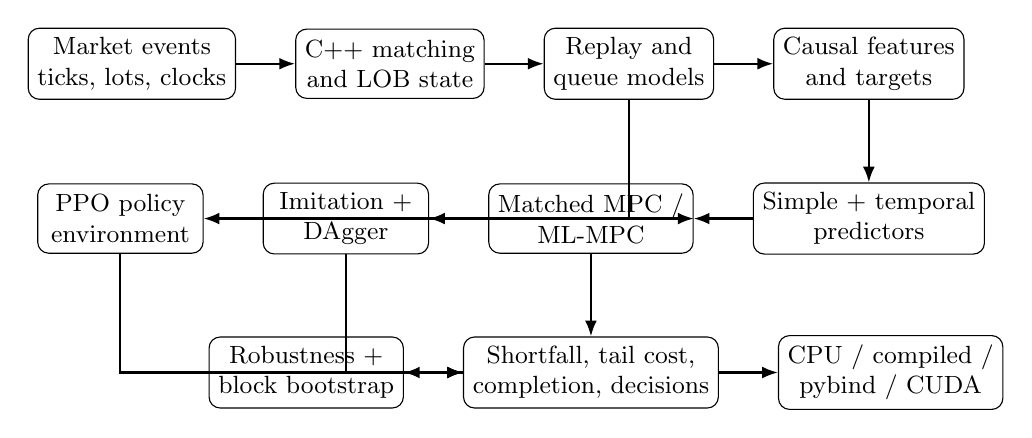
\begin{tikzpicture}[
    node distance=1.05cm and 0.75cm,
    box/.style={draw,rounded corners,align=center,minimum height=0.88cm,minimum width=2.1cm,font=\small},
    arr/.style={-{Latex[length=2mm]},thick},
    group/.style={draw,dashed,rounded corners,inner sep=5pt}
]
\node[box] (events) {Market events\\ticks, lots, clocks};
\node[box,right=of events] (lob) {C++ matching\\and LOB state};
\node[box,right=of lob] (queue) {Replay and\\queue models};
\node[box,right=of queue] (features) {Causal features\\and targets};
\node[box,below=of features] (pred) {Simple + temporal\\predictors};
\node[box,left=of pred] (mpc) {Matched MPC /\\ML-MPC};
\node[box,left=of mpc] (imit) {Imitation +\\DAgger};
\node[box,left=of imit] (rl) {PPO policy\\environment};
\node[box,below=of mpc] (metrics) {Shortfall, tail cost,\\completion, decisions};
\node[box,left=of metrics] (stats) {Robustness +\\block bootstrap};
\node[box,right=of metrics] (perf) {CPU / compiled /\\pybind / CUDA};
\draw[arr] (events)--(lob);
\draw[arr] (lob)--(queue);
\draw[arr] (queue)--(features);
\draw[arr] (features)--(pred);
\draw[arr] (pred)--(mpc);
\draw[arr] (queue)|-(mpc);
\draw[arr] (mpc)--(imit);
\draw[arr] (queue)|-(rl);
\draw[arr] (mpc)--(metrics);
\draw[arr] (imit)|-(metrics);
\draw[arr] (rl)|-(metrics);
\draw[arr] (metrics)--(stats);
\draw[arr] (metrics)--(perf);
\end{tikzpicture}
\caption{Research-system architecture. Market mechanics, causal prediction, decision policies, statistical analysis, and systems performance share the same execution-accounting layer.}
\label{fig:architecture}
\end{figure*}

\section{Experimental Design and Evaluation Protocol}
\label{sec:design}
The experimental design separates forecasting quality, controller behavior, sequential policy performance, robustness, statistics, and systems timing. This separation is intentional: a change in an upstream metric is not interpreted as economically valuable unless the downstream layer is evaluated directly.

\subsection{Evidence Tiers and Claim Boundary}
The evidence is divided before analysis into three tiers. Strategy conclusions use registered deterministic simulator populations so mechanisms can be isolated under identical random seeds. Systems conclusions use direct measurements on the CPU and Tesla T4 environments recorded with the artifacts. Historical-feed ingestion, sequence admission, and replay interfaces are implemented, but the locked historical strategy test remains unopened because no qualifying dataset has been admitted. Consequently, the paper makes no historical profitability or deployment-performance claim.

\begin{table}[t]
\centering
\caption{Evidence Tiers and Permitted Interpretation}
\label{tab:evidence-tiers}
\scriptsize
\setlength{\tabcolsep}{3pt}
\begin{tabular}{p{1.4cm}p{2.0cm}p{3.45cm}}
\toprule
Tier & Evidence & Permitted claim \\
\midrule
Controlled & registered simulator episodes & comparison within generator, controller, and stress assumptions \\
Systems & identified CPU/T4 measurements & workload- and hardware-specific performance \\
Historical & contracts only; test unopened & engineering readiness, not strategy performance \\
\bottomrule
\end{tabular}
\end{table}

\subsection{Controlled Populations and Split Discipline}
The microstructure-prediction experiment uses 100 chronological controlled day identifiers spanning BTCUSDT and ETHUSDT and both passive sides. The temporal sequence corpus contains 2,000 eight-step examples partitioned into 1,000 training, 400 validation, 200 calibration, and 400 untouched holdout sequences. Each candidate horizon uses the same split roles. Training fits weights and normalizers; validation chooses hyperparameters and stopping epoch; calibration estimates probability calibration; the holdout is evaluation-only.

Sequential execution experiments use independent episode populations rather than reusing the forecasting holdout. Imitation learning uses 80 training episodes, 30 validation episodes, 30 correction-pool episodes, 30 controlled-holdout episodes, and 30 OOD episodes, with six decisions per episode before environment-dependent termination. The RL experiment trains across three controlled regime families and evaluates on distinct ID and OOD regime sets. The Step-28 robustness matrix then reuses a fixed set of 24 paired episode seeds inside each stress cell so every policy experiences the same stochastic environment realization.

\begin{table}[t]
\centering
\caption{Primary Experimental Populations}
\label{tab:populations}
\scriptsize
\setlength{\tabcolsep}{2.8pt}
\resizebox{\columnwidth}{!}{%
\begin{tabular}{lll}
\toprule
Stage & Population & Role \\
\midrule
Temporal ML & 1000/400/200/400 seq. & train/val/cal/holdout \\
Imitation & 80/30/30/30/30 ep. & train/val/correct/holdout/OOD \\
PPO & 5 seeds & aggregate all seeds \\
Robustness & 43 $\times$ 24 paired ep. & stress evaluation \\
Statistics & 129 contrasts & block bootstrap \\
\bottomrule
\end{tabular}%
}
\end{table}

\subsection{Forecast Metrics}
For binary target $y_i$ and probability $p_i$, log loss and Brier score are
\begin{align}
\mathcal{L}_{\log} &=-\frac{1}{n}\sum_{i=1}^{n}\left[y_i\log p_i+(1-y_i)\log(1-p_i)\right],\\
\mathcal{L}_{\mathrm{Brier}} &=\frac{1}{n}\sum_{i=1}^{n}(p_i-y_i)^2.
\end{align}
Expected calibration error partitions predictions into bins $\mathcal{B}_m$ and computes
\begin{equation}
\mathrm{ECE}=\sum_m \frac{|\mathcal{B}_m|}{n}\left|\mathrm{acc}(\mathcal{B}_m)-\mathrm{conf}(\mathcal{B}_m)\right|.
\end{equation}
ROC-AUC and PR-AUC are retained because class prevalence differs sharply by horizon, but probability-sensitive metrics are central because the downstream MPC consumes probabilities rather than thresholded labels.

For the linear baseline,
\begin{equation}
p(y=1\mid x)=\sigma(w^\top x+b),
\end{equation}
and Platt calibration maps an uncalibrated logit $z$ to
\begin{equation}
p_{\mathrm{cal}}=\sigma(az+b_c),
\label{eq:platt}
\end{equation}
with $a,b_c$ fitted only on the calibration partition.

\subsection{Execution and Policy Metrics}
The primary economic measure is implementation shortfall in \cref{eq:is-bps}. Sequential evaluations additionally report completion rate, invalid-action rate, residual inventory, action frequencies, mean cost, p95 cost, and $\CVaR_{0.95}$. For episode costs $C_1,\ldots,C_n$, empirical tail cost is
\begin{equation}
\widehat{\CVaR}_{0.95}=\frac{1}{|\mathcal{T}|}\sum_{i\in\mathcal{T}} C_i,
\end{equation}
where $\mathcal{T}$ contains observations at or above the empirical 95th-percentile threshold. Imitation adds teacher-action agreement and fallback rate. Prediction-to-decision analysis reports whether a probability improvement changes the MPC action and whether the resulting execution cost changes.

\subsection{Selection and Ablation Discipline}
Model-family comparisons, calibration, controller sensitivity, imitation correction, and RL evaluation are separated by fixed data roles and configuration files. Neutral/base-rate controls test whether the ML controller collapses to the non-ML path; shuffled and stale predictions test dependence on signal information; a perfect intermediate-event oracle tests target-objective alignment; zero prediction weight tests solver equivalence. PPO reports all five registered seeds and the robustness matrix uses paired episode seeds. This design reduces the opportunity for post-hoc winner selection and makes negative or invariant results visible in the same artifacts as positive results.

\section{Classical Execution Policies and Receding-Horizon MPC}
\label{sec:mpc}
\subsection{Baselines}
The baseline family contains immediate execution, a time-sliced TWAP-like schedule, a liquidity-aware policy, and an Almgren--Chriss-style control benchmark. Immediate execution establishes the cost of maximal urgency. TWAP-like execution distributes quantity over the horizon. The liquidity-aware policy conditions aggressiveness on visible spread/depth and remaining inventory. These baselines are intentionally strong enough that an RL or ML controller must improve a meaningful comparator rather than a trivial policy.

\subsection{Queue-Aware Local Fill Proxy}
The non-ML MPC uses a bounded local passive-fill proxy to rank candidate action sequences inside a short solve. Let $Q_s$ and $Q_o$ denote same- and opposite-side top-level depth and $F\in[0,1]$ a normalized flow signal. The queue-share term is
\begin{equation}
q_{\mathrm{share}}=\frac{Q_s}{Q_s+Q_o},
\end{equation}
and the local proxy is
\begin{equation}
\hat p_{\mathrm{fill}} = \clip\left(p_0+w_q(0.5-q_{\mathrm{share}})+w_f(F-0.5),0,1\right).
\label{eq:fill-proxy}
\end{equation}
This quantity is a controller heuristic, not a learned probability model. It is held fixed within a local search and recomputed after the environment advances.

\subsection{Finite-Horizon Search}
The MPC enumerates a bounded action tree with planning horizon at most four, action fractions $\{1/4,1/2,1\}$, and maximum passive fraction $1/2$. Only the first action of the lowest-cost plan is executed; the state is then observed again and the optimization repeats. This receding construction limits open-loop sensitivity.

For a candidate stage $k$, a generic cost is
\begin{equation}
J_k = C_{\mathrm{exec},k} + \lambda_I \left(\frac{I_{k+1}}{Q}\right)^2 + J_{k+1},
\end{equation}
where an aggressive branch uses visible-sweep cost plus fees and depth penalties, while a passive branch uses expected attempted fill under \cref{eq:fill-proxy}. The terminal cost is
\begin{equation}
J_T = \frac{I_T}{Q}\left(C_{\mathrm{forced}}+\lambda_T\right)
+\lambda_Q\left(\frac{I_T}{Q}\right)^2.
\label{eq:terminal}
\end{equation}
The central controller parameters use $\lambda_I=2\bps$, $\lambda_T=20\bps$, and $\lambda_Q=10\bps$. These terms do not replace exact accounting; they only shape the optimizer's action choice.

\begin{algorithm}[t]
\caption{Receding-Horizon Execution Control}
\label{alg:mpc}
\DontPrintSemicolon
\KwIn{causal observation $x_k$, remaining inventory $I_k$}
Build bounded candidate action tree $\mathcal{T}(x_k,I_k)$\;
Evaluate passive branches using queue state and local fill proxy\;
Evaluate aggressive branches by visible sweep and fee/impact terms\;
Add inventory-risk and terminal-completion costs\;
$a_k \leftarrow$ first action of lowest-cost path\;
Validate $a_k$ against inventory and market constraints\;
Execute $a_k$, advance environment, observe $x_{k+1}$\;
Repeat until $I_k=0$ or terminal completion\;
\end{algorithm}

\section{Causal Microstructure Prediction}
\label{sec:prediction}
\subsection{Target Definition}
For each candidate horizon $h\in\{250\text{ ms},1\text{ s},5\text{ s}\}$, the primary binary target is same-side best-quote depletion or trade-through within $h$. If the passive side at decision time is $d\in\{\mathrm{bid},\mathrm{ask}\}$, the target can be written
\begin{align}
y_h(t)=\1\{&\text{same-side best quote depletes} \nonumber\\
             &\text{or is traded through in }(t,t+h]\}.
\label{eq:target}
\end{align}
A side-signed adverse-move target is retained as a secondary diagnostic. The primary target is deliberately described as a quote-depletion/trade-through event; it is not algebraically identified with the realized fill of a specific child order.

\subsection{Causal Information Contract}
Let a decision occur at wall-clock time $t$ and let the market observation cutoff be
\begin{equation}
c=t-\ell_{\mathrm{obs}},
\end{equation}
where $\ell_{\mathrm{obs}}$ is observation latency. A source event $e$ can contribute to the feature vector only if
\begin{equation}
t_e\le c \quad \text{and}\quad t^{\mathrm{available}}_e\le t.
\label{eq:causality}
\end{equation}
This dual-time rule prevents both future-event leakage and availability-time leakage. Mutation tests perturb events after the cutoff and require the frozen feature vector to remain unchanged.

\subsection{Frozen Feature Set}
The feature contract contains 20 causal variables, grouped as follows:
\begin{itemize}[leftmargin=*]
    \item \textbf{spread/depth:} spread in ticks; same/opposite top-1 lots; same/opposite top-5 lots;
    \item \textbf{imbalance:} side-aligned top-1 and top-5 imbalance in basis-point-scaled units;
    \item \textbf{trade flow:} toward-quote signed trade flow over 250~ms, 1~s, and 5~s; trade counts over 1~s and 5~s;
    \item \textbf{price dynamics:} side-aligned mid moves over 250~ms, 1~s, and 5~s; realized absolute mid movement over 1~s and 5~s; 1~s spread change;
    \item \textbf{staleness:} quote age and time since last trade.
\end{itemize}
Exact names and units are reproduced in Appendix~\ref{app:features}.

\subsection{Simple Model Ladder and Calibration}
Each horizon is first modeled by a deliberately compact ladder: training base rate, L2-regularized logistic regression, histogram gradient-boosted trees, and a one-hidden-layer MLP. Logistic and MLP inputs use a scaler fitted on training data only. Hyperparameters are selected on validation data; Platt scaling is fitted on a separate calibration partition. Metrics include log loss, Brier score, expected calibration error, calibration slope/intercept, ROC-AUC, PR-AUC, and temporal/instrument/passive-side slices.

\subsection{Temporal Model}
The temporal predictor consumes an eight-step causal history $X\in\R^{8\times20}$. The architecture is
\begin{equation}
X \xrightarrow{\mathrm{causal\ Conv1D}(k=3)} H_c
\xrightarrow{\mathrm{GELU}} H_g
\xrightarrow{\mathrm{LSTM}} h_8
\xrightarrow{\mathrm{linear}} z,
\label{eq:temporal}
\end{equation}
followed by probability $\sigma(z)$ and optional Platt transform $\sigma(az+b)$. Left padding preserves causality. The controlled dataset contains 4,800 source rows and 2,000 sequences split into 1,000 training, 400 validation, 200 calibration, and 400 controlled-holdout sequences. The scaler is fitted on training only; early stopping uses validation only; calibration uses calibration only.

\begin{table}[t]
\centering
\caption{Temporal Model Configurations}
\label{tab:temporal-config}
\begin{tabular}{lrrrr}
\toprule
Horizon & Conv & LSTM & Params. & Epoch \\
\midrule
250 ms & 12 & 12 & 1,993 & 3 \\
1 s    & 8  & 8  & 1,073 & 4 \\
5 s    & 12 & 12 & 1,993 & 5 \\
\bottomrule
\end{tabular}
\end{table}
All configurations use AdamW, learning rate $5\times10^{-3}$, weight decay $10^{-4}$, gradient clipping, deterministic CPU training, no dropout, maximum 14 epochs, and patience 3. Training prevalences are 4.5\%, 17.8\%, and 58.9\% for 250~ms, 1~s, and 5~s respectively.

\section{ML-Assisted MPC and Prediction-to-Decision Analysis}
\label{sec:mlmpc}
\subsection{Matched Controller Construction}
The ML-assisted controller reuses the exact same finite-horizon search, action space, queue model, latency model, aggressive-cost implementation, inventory penalty, and terminal handling as the non-ML MPC. The intended difference is a prediction-derived passive-risk adjustment. For predicted event probability $p$ and training base rate $\bar p$, the additive adjustment is
\begin{equation}
\Delta C_{\mathrm{pred}} = \lambda_p(p-\bar p),
\label{eq:prediction-term}
\end{equation}
where $\lambda_p$ is a controlled sensitivity weight in basis points. Centering at the base rate creates an exact neutral control: replacing every prediction by $\bar p$ produces zero adjustment at every decision. Setting $\lambda_p=0$ separately verifies that the ML path reduces byte-for-byte to the non-ML decision accounting in the deterministic fixture.

Every prediction endpoint carries decision identifier, endpoint time, feature cutoff, availability time, horizon, model identifier, provenance identifier, probability, base rate, and prediction kind. The controller rejects duplicate, unavailable, future, or mismatched endpoints rather than substituting a default probability.

\subsection{Ablation Design}
The registered inputs are calibrated model probability, uncalibrated model probability, training base rate, within-day/instrument shuffled predictions, stale predictions, a perfect intermediate-event oracle, and zero prediction weight. Decision sensitivity is evaluated on
\begin{multline}
\lambda_p\in\{0,50,100,250,500,1000,\\
2000,5000,10000,25000\}\bps.
\end{multline}
This separates three questions: whether a predictor is statistically better, whether its output changes the controller, and whether the changed action improves downstream execution cost.

\subsection{Predictive Results}
\begin{table}[t]
\centering
\caption{Controlled-Holdout Log Loss and Controller Sensitivity}
\label{tab:pred-results}
\begin{tabular}{lrrrr}
\toprule
Horizon & Base & Raw & Cal. & First change$^\dagger$ \\
\midrule
250 ms & 0.1453 & \textbf{0.1442} & 0.1618 & 5,000 / none \\
1 s    & 0.4829 & \textbf{0.4738} & 0.4780 & none / none \\
5 s    & 0.6895 & 0.6675 & \textbf{0.6401} & 10,000 / 5,000 \\
\bottomrule
\multicolumn{5}{l}{\footnotesize $^\dagger$calibrated / uncalibrated prediction-weight threshold in bps.}
\end{tabular}
\end{table}

\Cref{tab:pred-results,fig:pred-quality} show a non-monotonic mapping. At 5~s, calibration improves log loss from 0.6675 to 0.6401, yet the uncalibrated signal changes the controller at a lower sensitivity weight. At 250~ms, calibration worsens log loss but can still cross a decision boundary at high weight while the raw signal does not. At 1~s, both learned variants improve on the base-rate log loss, but neither changes the controller anywhere on the registered grid.

\begin{figure}[t]
\centering
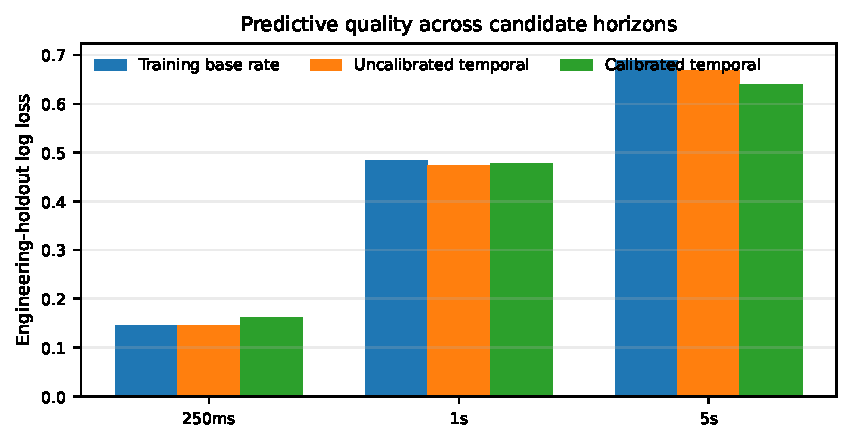
\includegraphics[width=\columnwidth]{prediction_logloss.pdf}
\caption{Predictive quality across candidate horizons on the 400-sequence controlled holdout per horizon. Lower log loss is better.}
\label{fig:pred-quality}
\end{figure}

Across the registered comparison-weight cases, prediction and decision outcomes decompose into 84 cases in which prediction improves but the decision is unchanged, 26 in which both improve/change, 32 in which prediction does not improve and the decision is unchanged, and 8 in which prediction does not improve yet the decision changes. \Cref{fig:pred-decision} visualizes this separation.

\begin{figure}[t]
\centering
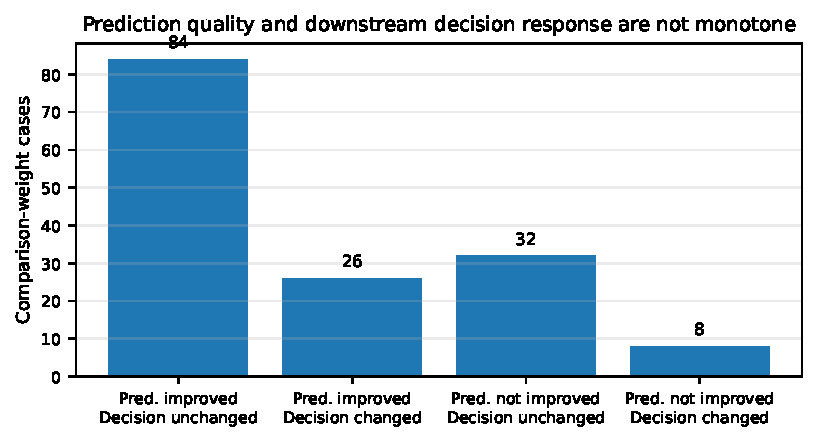
\includegraphics[width=\columnwidth]{prediction_decision_relationships.pdf}
\caption{Relationship between predictive improvement and downstream action response. The optimizer often absorbs prediction changes without changing its first action.}
\label{fig:pred-decision}
\end{figure}

A particularly useful diagnostic is the perfect event oracle. It predicts the intermediate quote-depletion/trade-through target without classification error, yet can still worsen implementation shortfall in the controlled execution fixture. This demonstrates that an oracle for an intermediate microstructure target is not an oracle for the execution objective. The result motivates explicit decision-value evaluation and, potentially, future decision-focused training.

\section{Imitation Learning for Low-Latency Policy Approximation}
\label{sec:imitation}
\subsection{Teacher Construction}
A first behavior-cloning attempt exposed a degenerate teacher action surface: under the conservative non-ML MPC configuration, nearly all sampled controlled states selected the same first action. Rather than accepting a misleadingly high imitation accuracy, the teacher-data generator was expanded over controlled state dimensions and uses the already validated shared MPC optimizer with a causal controlled prediction-risk input to expose multiple optimizer action classes.

The training teacher distribution contains 480 labeled states with class counts 297 passive-50, 162 aggressive-100, 19 aggressive-50, and 2 aggressive-25. The C++ teacher oracle returns both the exact MPC action and adaptive signal vector for arbitrary causal states, which allows expert relabeling on learner-visited states.

\subsection{Behavior Cloning and DAgger}
The student is a one-hidden-layer MLP. Validation-only model selection chooses eight hidden units and L2 regularization $\alpha=10^{-4}$. Let $\pi_T$ be the teacher and $\pi_\theta$ the student. Initial behavior cloning minimizes categorical cross-entropy
\begin{equation}
\mathcal{L}_{\mathrm{BC}}(\theta)=-\sum_{(x,a)\in\mathcal{D}}\log \pi_\theta(a\mid x).
\end{equation}
A predeclared sequential validation agreement threshold of 98\% determines whether correction is required. The initial student achieves 97.70\%, triggering one DAgger-style correction round. Learner rollouts over a dedicated correction pool generate visited states $x\sim d_{\pi_\theta}$, the C++ oracle labels $a=\pi_T(x)$, and 87 corrective examples are appended before retraining.

After correction, validation agreement increases to 98.84\%. On the untouched controlled holdout, the student reproduces the teacher action path exactly, with 100\% action agreement, 100\% completion, zero invalid actions, and zero shortfall delta relative to the teacher.

\subsection{Out-of-Distribution Behavior and Fallback}
OOD regimes intentionally shift liquidity, volatility, latency, and execution parameters. Raw student agreement falls to 69.30\%, and p95 implementation shortfall increases to 455\bps versus 281.45\bps for the teacher. A validation-selected conservative fallback sends uncertain states back to the teacher and raises agreement to 94.78\%, with p95 shortfall 287.5\bps. The fallback is invoked on 82.61\% of OOD decisions, exposing the latency-versus-robustness trade-off directly.

\begin{figure}[t]
\centering
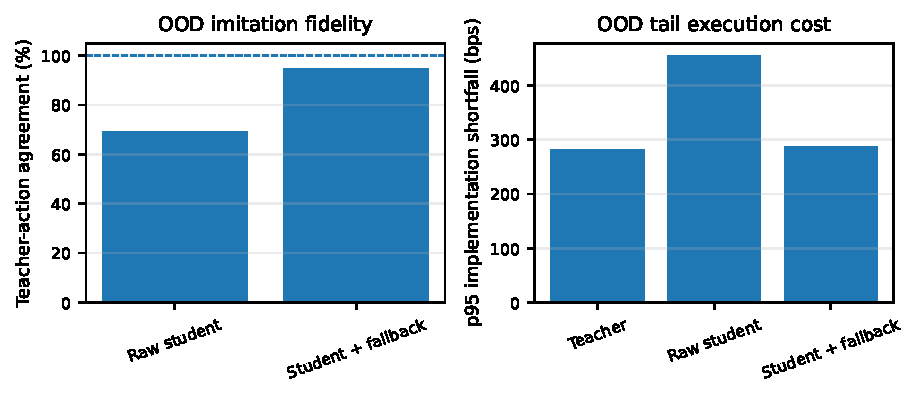
\includegraphics[width=\columnwidth]{imitation_ood.pdf}
\caption{OOD imitation behavior. A validation-selected teacher fallback recovers most action fidelity and tail-cost behavior, but at a high fallback rate.}
\label{fig:imit-ood}
\end{figure}

\section{Reinforcement Learning Environment and PPO}
\label{sec:rl}
\subsection{Markov Decision Process}
The controlled execution environment exposes an 11-dimensional causal state: remaining-inventory fraction, time remaining, scaled spread, depth ratio, imbalance, volatility, latency, fee, impact coefficient, recent fill, and adverse momentum. The action set is given by \cref{eq:rl-actions}. Episodes contain 12 decision steps and a parent size of 100 lots in the central configuration. Action masks prevent terminal or inventory-infeasible decisions.

The environment is interactive rather than a static classifier: aggressive participation induces temporary impact on subsequent state transitions. Training regimes cover normal, active, and thin liquidity. OOD evaluation includes thin/high-volatility, high-latency, adverse-fee, high-impact, and combined regimes.

\subsection{Reward Accounting}
For each transition, the environment stores raw fill price, fill quantity, visible depth, arrival price, fee, latency, impact, adverse-momentum input, inventory before action, and terminal-fill information. The reward is
\begin{equation}
r_k=-\left(C_{\mathrm{fill},k}+\lambda_I\left(\frac{I_{k+1}}{Q}\right)^2+C_{\mathrm{terminal},k}\right).
\label{eq:reward}
\end{equation}
A separate reconstruction function recomputes the economic cost from the raw transition facts. The deterministic reward audit obtains absolute reconstruction error 0.0. Additional tests verify that terminal inventory cannot disappear, executed quantity cannot exceed the parent order, invalid actions are masked consistently, and future random draws cannot alter the current observation.

\subsection{PPO Objective and Configuration}
The policy uses two 32-unit $\tanh$ hidden layers with a categorical action head and value head. With probability ratio
\begin{equation}
r_t(\theta)=\frac{\pi_\theta(a_t\mid s_t)}{\pi_{\theta_{\mathrm{old}}}(a_t\mid s_t)},
\end{equation}
PPO optimizes the clipped objective \cite{SchulmanWolskiDhariwalRadfordKlimov2017}
\begin{equation}
L^{\mathrm{clip}}(\theta)=\E_t\left[\min\left(r_t(\theta)\hat A_t,\clip(r_t(\theta),1-\epsilon,1+\epsilon)\hat A_t\right)\right].
\label{eq:ppo}
\end{equation}
The registered configuration uses $\gamma=0.99$, GAE $\lambda=0.95$, clipping $\epsilon=0.2$, entropy coefficient 0.01, value coefficient 0.5, learning rate $10^{-3}$, 20 training episodes per update, four update epochs, and ten updates. Five independent seeds $\{27,127,227,327,427\}$ are all retained.

\subsection{Multi-Seed Results}
\begin{table}[t]
\centering
\caption{Controlled RL Evaluation (Lower Cost Is Better)}
\label{tab:rl-results}
\footnotesize
\setlength{\tabcolsep}{2.6pt}
\begin{tabular}{lrrrr}
\toprule
Policy & ID $\mu$ & ID C95 & OOD $\mu$ & OOD C95 \\
\midrule
PPO (5 seeds) & 1.214 & 11.942 & 7.333 & 26.961 \\
Liquidity-aware & \textbf{0.820} & 11.026 & 8.554 & 23.559 \\
TWAP-like & 2.488 & 7.272 & \textbf{7.004} & \textbf{17.821} \\
Immediate & 3.879 & \textbf{6.649} & 13.442 & 33.069 \\
\bottomrule
\end{tabular}
\end{table}
The PPO aggregate achieves 100\% completion and zero invalid-action rate across registered ID and OOD evaluation episodes, but it is not uniformly lowest cost. Liquidity-aware execution has lower ID mean cost, while TWAP-like execution has lower OOD mean and OOD CVaR95. PPO seed variation is material: ID mean cost ranges approximately from 0.20 to 3.34\bps across the five registered seeds. This is precisely why the aggregate and all seeds are retained rather than reporting a best run.

\begin{figure}[t]
\centering
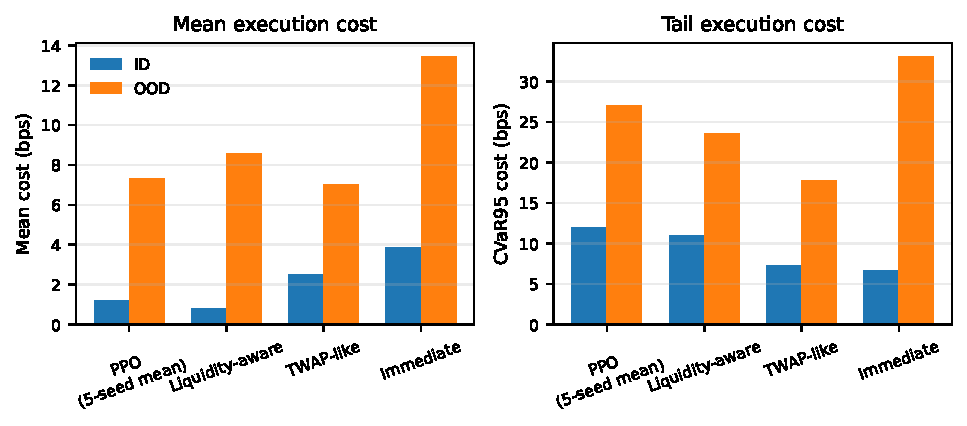
\includegraphics[width=\columnwidth]{rl_id_ood.pdf}
\caption{Mean and tail execution cost for PPO and strong deterministic baselines in controlled ID/OOD evaluation.}
\label{fig:rl-results}
\end{figure}

\section{Robustness Matrix}
\label{sec:robustness}
A robust execution policy should not be selected from a single central configuration. The robustness experiment therefore evaluates 43 registered stress cells, each using the same 24 paired episode seeds for all comparable policies. Dimensions include observation latency, decision-grid resolution, visible liquidity, spread, volatility, aggregate-L2 queue assumptions, fees/rebates, parent-order size, horizon, impact magnitude and functional form, prediction degradation, data drop/delay, temporal/instrument distribution shift, compute constraints, and simulator mismatch.

\subsection{Ranking Changes}
The central regime mean costs are 2.232\bps for liquidity-aware, 2.514\bps for PPO aggregate, 3.123\bps for TWAP-like, and 3.947\bps for immediate execution. Across all 43 cells, liquidity-aware ranks first in 35, PPO aggregate in 5, TWAP-like in 3, and immediate in none. More importantly, the identity or ordering of strategies changes in 16 of the 42 non-central cases.

\begin{figure}[t]
\centering
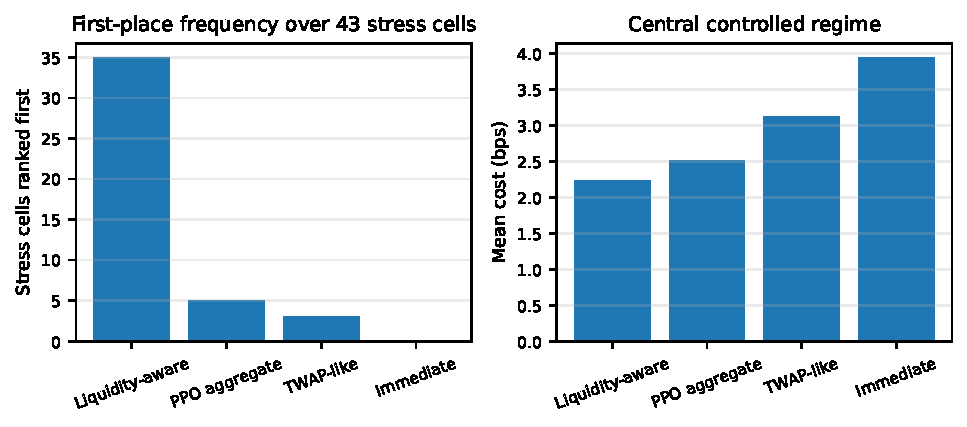
\includegraphics[width=\columnwidth]{robustness_summary.pdf}
\caption{Robustness summary: first-place frequency across 43 stress cells and central-regime mean execution cost.}
\label{fig:robustness-summary}
\end{figure}

The stress matrix reveals qualitatively different failure modes. Under a volatility shock, mean costs are approximately 0.824\bps (liquidity-aware), 3.202\bps (TWAP-like), 4.397\bps (immediate), and 6.988\bps (PPO). Under the combined unseen regime they become 12.182, 13.363, 32.511, and 18.044\bps respectively. In one adverse simulator-mismatch cell, however, PPO becomes the point winner at 4.667\bps, narrowly ahead of TWAP-like at 4.737\bps and liquidity-aware at 5.913\bps. Thus robustness is regime-dependent rather than reducible to a single policy ranking.

Worst mean-cost increases relative to the central regime are approximately +28.56\bps for immediate, +15.53\bps for PPO aggregate, +10.24\bps for TWAP-like, and +9.95\bps for liquidity-aware. These values quantify sensitivity rather than merely counting wins.

\section{Dependence-Aware Statistical Analysis}
\label{sec:stats}
\subsection{Paired Contrasts}
Every comparable stress cell uses paired episode seeds, so inference is performed on paired cost differences rather than independent policy samples. If $C_{i,A}$ and $C_{i,B}$ are costs for paired episode $i$, the effect variable is
\begin{equation}
d_i=C_{i,A}-C_{i,B}.
\end{equation}
Positive values imply higher cost for $A$.

\subsection{Moving-Block Bootstrap}
To avoid treating ordered pseudo-day observations as IID, the controlled analysis uses a moving-block bootstrap. A frozen autocorrelation rule selects block length $L=5$: the relevant paired-difference autocorrelation remains below $|\rho|<0.1$ for two consecutive lags beginning at lags 5 and 6. Each registered contrast uses $B=4096$ bootstrap replications. A bootstrap sample concatenates contiguous blocks while preserving the within-episode policy pairing.

For statistic $\hat\theta$, the empirical percentile interval is
\begin{equation}
\left[\hat\theta^{*(\alpha/2)},\hat\theta^{*(1-\alpha/2)}\right], \qquad \alpha=0.05.
\end{equation}
Exploratory stress families use Holm step-down multiplicity adjustment \cite{RomanoWolf2005}. In addition to pairwise effects, a ranking bootstrap resamples the common paired observations and recomputes the lowest-cost policy, producing a probability that the point-estimate winner remains first.

\subsection{Uncertainty Results}
There are 129 paired controlled contrasts. Of these, 85 have 95\% intervals crossing zero. Of the 43 stress-cell point winners, 21 achieve at least 80\% bootstrap probability of remaining best and 22 do not. The central point winner, liquidity-aware, has bootstrap win probability 87.84\%; PPO aggregate has 8.13\%, TWAP-like 2.22\%, and immediate 1.81\%.

For the central PPO-minus-liquidity-aware contrast, the mean paired difference is approximately +0.282\bps with 95\% interval $[-0.106,0.658]\bps$. The point ranking therefore contains substantial uncertainty even though the mean costs differ. Several apparent PPO/TWAP point wins are more fragile: the 25\%-depth PPO winner retains only approximately 39.5\% bootstrap win probability, while narrow-spread TWAP and selected simulator-mismatch PPO wins remain below 50\%.

\begin{figure}[t]
\centering
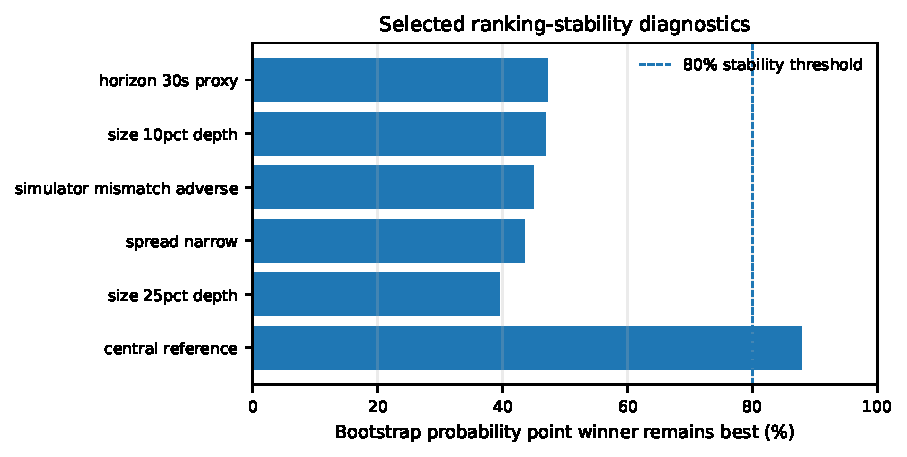
\includegraphics[width=\columnwidth]{ranking_stability_selected.pdf}
\caption{Bootstrap probability that selected stress-cell point winners remain lowest cost. The dashed line marks the preregistered 80\% ranking-stability diagnostic.}
\label{fig:ranking-stability}
\end{figure}

This analysis changes the interpretation of the robustness table: first-place counts summarize observed point estimates, while the bootstrap quantifies how often those rankings survive paired resampling.

\section{High-Performance Systems Evaluation}
\label{sec:performance}
Execution logic operates under tight decision budgets, so compute latency is treated as an execution-system variable. The performance study follows a profile-first workflow: measure a representative workload, identify a concrete bottleneck, apply one narrow optimization, rerun correctness, and then benchmark scaling.

\subsection{C++ Matching Engine}
The microbenchmark repeatedly rests and immediately matches orders through the real C++ matching engine, with 60,000 submit operations per repetition. Profiling identifies measurable unordered-map growth and rehashing overhead. The optimization adds an optional expected-order-count capacity hint that reserves identifier/history tables in advance. The default remains zero, preserving prior allocation behavior. A direct regression requires the hinted and unhinted engines to produce identical canonical book state and deterministic checksum.

\begin{table}[t]
\centering
\caption{C++ Matching Benchmark}
\label{tab:cpp-perf}
\begin{tabular}{rrrrr}
\toprule
Threads & Base ms & Opt. ms & Speedup & Opt. Mops/s \\
\midrule
1 & 13.527 & 13.286 & 1.018$\times$ & 4.516 \\
2 & 6.895 & 6.591 & 1.046$\times$ & 9.103 \\
4 & 4.932 & 3.465 & 1.423$\times$ & 17.316 \\
\bottomrule
\end{tabular}
\end{table}
The process-level 100k-pair memory check is effectively flat: measured maximum resident set size is approximately 49,544~KiB before and 49,128~KiB with the capacity hint. The optimization therefore targets rehash work without introducing a material memory expansion in the measured workload.

\begin{figure}[t]
\centering
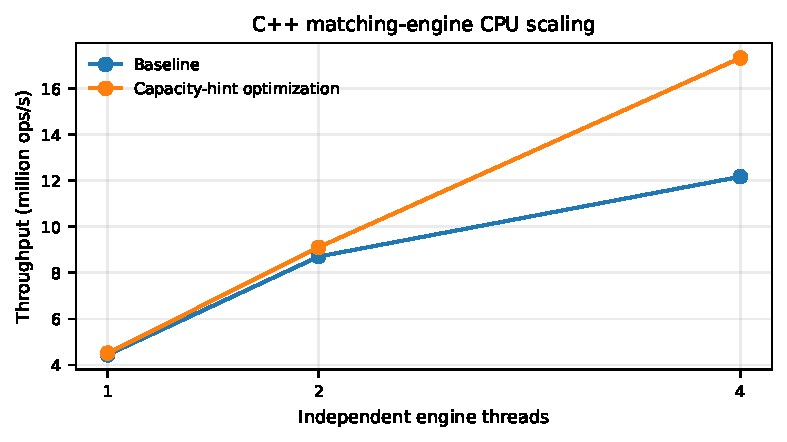
\includegraphics[width=\columnwidth]{cpp_scaling.pdf}
\caption{Measured C++ matching throughput for independent engines as thread count increases.}
\label{fig:cpp-scaling}
\end{figure}

\subsection{CPU Neural Inference}
The primary CPU benchmark host exposes five AMD EPYC 9V74 logical/physical CPUs, approximately 6.37~GB memory, GCC 14.2, Python 3.13.5, NumPy 2.3.5, scikit-learn 1.8.0, and PyTorch 2.10.0+cpu. Batch-one and batched inference are measured separately because low-latency decisions and offline throughput are different workloads.

For the imitation policy, the measured batch-one median is 11.88~$\mu$s in NumPy and 9.84~$\mu$s through the traced PyTorch compatibility path; at batch 256 the traced path reaches approximately 9.54 million rows/s. For PPO, batch-one eager inference is approximately 31.15~$\mu$s in the primary CPU benchmark and the traced path approximately 15.84~$\mu$s; at batch 256 it reaches approximately 3.13 million rows/s. The temporal model benefits strongly from batching, reaching hundreds of thousands of rows/s depending on thread count.

Current PyTorch compiler paths are measured separately from deprecated compatibility paths. The temporal LSTM can be captured with \texttt{torch.export}; full-graph \texttt{torch.compile} is unsupported for the measured recurrent path, while graph-break compilation is slower at batch one. This distinction prevents a fast legacy trace measurement from being mistaken for a future deployment recommendation.

\subsection{Python--C++ Boundary}
The existing binding is built against pybind11-compatible headers and verified by an exact diagnostic-sequence equality check before timing. For the small diagnostic call, the C++ path through pybind has median 304.05~ns (p95 311.97~ns), compared with 1,748.6~ns (p95 1,761.3~ns) for the pure-Python reference. This microbenchmark isolates call-boundary overhead; it is not interpreted as an end-to-end simulator speedup.

\subsection{Transfer-Inclusive CUDA Benchmark}
The CUDA experiment runs on a Google Colab Tesla T4 (compute capability 7.5) with PyTorch 2.11.0+cu128 and CUDA 12.8. Before accepting timings, CPU and GPU outputs are compared for numerical equivalence. Both GPU-resident and transfer-inclusive timings are recorded. The transfer-inclusive path explicitly includes CPU-to-GPU input movement, inference, synchronization, and result movement back to CPU.

\begin{table}[t]
\centering
\caption{Tesla T4 Transfer-Inclusive Inference}
\label{tab:cuda}
\begin{tabular}{lrrr}
\toprule
Workload & Batch & CPU $\mu$s & T4 $\mu$s \\
\midrule
Imitation & 1 & 28.68 & 181.70 \\
PPO & 1 & 69.96 & 341.24 \\
Temporal 5 s & 1 & 485.85 & 662.06 \\
Temporal 5 s & 32 & 682.17 & 713.58 \\
Temporal 5 s & 256 & 1281.69 & \textbf{752.35} \\
\bottomrule
\end{tabular}
\end{table}
At batch one, transfer-inclusive GPU execution is slower for every registered workload. For the temporal model at batch 256, GPU becomes advantageous with measured speedup
\begin{equation}
S_{256}=\frac{1281.69}{752.35}\approx1.704\times.
\end{equation}
Maximum output-equivalence error is 0 for the imitation and PPO workloads and approximately $10^{-6}$ for the temporal model.

\begin{figure}[t]
\centering
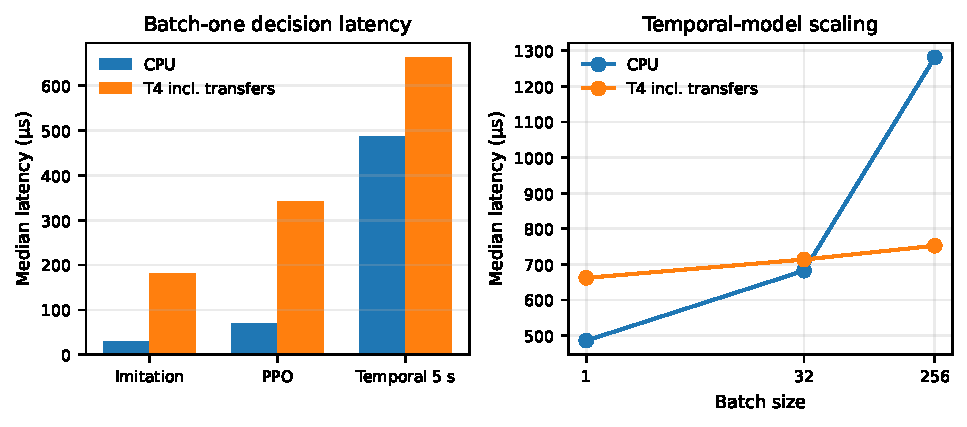
\includegraphics[width=\columnwidth]{cuda_performance.pdf}
\caption{CPU versus transfer-inclusive Tesla T4 inference. The latency-sensitive batch-one path favors CPU, while temporal inference becomes GPU-favorable at large batch.}
\label{fig:cuda}
\end{figure}

\section{Discussion}
\label{sec:discussion}
\subsection{Prediction Quality Is Not Decision Quality}
The strongest recurring result is the non-monotonic mapping from probability metrics to execution decisions. A predictor can improve log loss without crossing an MPC decision boundary, while a less accurate or less calibrated signal can cross a boundary because its probability mass is distributed differently around the controller's effective threshold. The perfect-event-oracle experiment strengthens this interpretation: even exact knowledge of the intermediate quote-depletion target need not improve implementation shortfall. The economic objective depends on inventory, spread, queue uncertainty, urgency, terminal cost, and the alternative action sequence, not on the target alone.

This observation suggests that forecasting benchmarks should be reported alongside downstream action/value diagnostics whenever the forecast is consumed by an optimizer. It also motivates future decision-focused loss functions that weight errors by their local execution consequence rather than their standalone probability score.

\subsection{Policy Complexity and Robustness}
The deterministic liquidity-aware heuristic remains highly competitive. PPO produces good controlled ID mean cost and wins selected stress cells, but it does not dominate the simpler baselines and degrades under particular volatility/OOD regimes. This is consistent with the generalization concerns emphasized in recent RL execution work \cite{ZhangDuanChen2023}. The result is not an argument against RL; rather, it shows that the burden of proof for an RL execution policy should include strong baselines, multiple seeds, OOD regimes, reward audits, and tail-risk metrics.

The imitation experiment provides a complementary lesson. A small student can exactly reproduce a teacher on an in-distribution holdout and offer very low inference latency, yet still fail under shifted states. DAgger-style correction improves sequential agreement, while conservative fallback controls OOD tail cost at the price of invoking the expensive teacher frequently. In a practical system, fallback rate therefore becomes an explicit systems metric alongside action agreement.

\subsection{Statistical Ranking Versus Point Ranking}
The 43-cell robustness table is informative but insufficient on its own. More than half of the 129 paired confidence intervals cross zero, and 22 of 43 point winners fall below the 80\% bootstrap ranking-stability diagnostic. This is a concrete example of why large strategy tables can create false confidence when each cell is interpreted independently. Paired resampling and family-wise multiplicity adjustment reveal which differences are robust enough to support stronger interpretation.

\subsection{Latency as Part of the Decision Problem}
The systems results reject the assumption that a GPU is automatically the correct inference platform for ML-assisted execution. For batch-one policies, the networks are so small that launch, synchronization, and host-device transfer dominate arithmetic. The T4 only becomes favorable for the temporal model at batch 256. The appropriate deployment architecture is therefore workload-dependent: CPU for latency-sensitive individual decisions; GPU for large batched temporal scoring or offline research workloads. Similar reasoning applies to compiler choices and language boundaries: an optimization is useful only after measuring the complete path that actually participates in the control loop.

\subsection{Threats to Validity and Research Boundary}
\textit{Construct validity:} The quote-depletion target is an intermediate microstructure event, not execution utility. The oracle counterexample demonstrates this mismatch directly. Implementation shortfall and terminal completion are therefore computed from realized fills under common accounting, but they remain conditional on the registered benchmark and cost model.

\textit{Internal validity:} Matched controllers, paired seeds, causal cutoffs, independent split roles, exact accounting, and zero-weight equivalence reduce confounding. Aggregate-L2 queue allocation, impact, and synthetic order flow are nevertheless scenario assumptions rather than estimated true-market parameters; the robustness matrix varies them but cannot eliminate misspecification.

\textit{Statistical validity:} Each stress cell contains 24 paired episodes, PPO uses five registered seeds, and the moving-block bootstrap operates on synthetic episode seeds as pseudo-days. Confidence intervals and ranking probabilities quantify sampling uncertainty in this design, but they do not establish universal policy ordering or substitute for a larger historical panel.

\textit{External validity:} Controlled state transitions isolate mechanisms but do not reproduce all hidden liquidity, exchange-specific priority rules, network jitter, outages, endogenous impact, or participant adaptation. Only one compact temporal architecture and one predeclared PPO family are evaluated; no architecture novelty or universal superiority is claimed. Any venue or historical regime is a new external-validity test.

\textit{Systems validity:} CPU and CUDA results are hardware- and workload-specific process measurements, not exchange round-trip latency or high-frequency deployment guarantees. The transfer-inclusive boundary is measured, but production networking, colocated exchange gateways, and operational failover lie outside scope. These boundaries leave a clear confirmatory next step: admit a qualifying multi-day historical dataset under the frozen Gate-C protocol and repeat the matched comparison without revising the hypothesis after observing outcomes.

\section{Reproducibility and Software Verification}
\label{sec:repro}
The research system is built as staged, schema-validated software rather than a single notebook. Deterministic artifacts carry hashes and provenance identifiers; model weights use canonical serialization where practical; experiment configurations are versioned; and validators regenerate committed outputs byte-for-byte when scientific determinism is meaningful.

The native inventory contains 53 tests and reports 53/53 passes in each registered compiler or sanitizer matrix: GCC, Clang, AppleClang, optimized Release, ASan/UBSan, and ThreadSanitizer. Compiler warnings are errors. The Python inventory contains 480 tests with 91\% combined branch-aware repository coverage. Independent semantic validators check data contracts, feature causality, model artifacts, controller equivalence, imitation/RL reports, robustness statistics, performance evidence, and the manuscript's headline claims. Expensive regeneration suites are partitioned rather than hidden behind a monolithic command timeout.

The final source tree additionally provides CMake packaging, an external consumer check, Docker/reproduction entry points, JSON Schemas for stage outputs, checksum manifests, a citation file, and a claim-to-artifact traceability table. The 566/566-file repository contract and release validator are automated in CI. Source, configurations, paper, figures, and evidence are publicly available at \url{https://github.com/000zer000/robust-ml-optimal-execution}; the paper can be rebuilt with one documented Tectonic target. This structure follows the general reproducibility principle that a computational result should be accompanied by sufficiently precise code, configuration, seeds, and compute information to make regeneration auditable \cite{PineauVincentLamarreSinhaLariviere2021}.

\section{Conclusion}
This paper presented an integrated framework for studying robust machine-learning-assisted optimal execution at the intersection of quantitative finance, market microstructure, machine learning, sequential control, and high-performance systems. The system begins with exact C++ event and matching semantics, models aggregate-L2 queue uncertainty explicitly, computes implementation shortfall from realized fills, and uses matched receding-horizon controllers to isolate the incremental effect of microstructure forecasts. It then extends the decision stack through calibrated temporal prediction, prediction-versus-decision ablations, imitation learning with DAgger, multi-seed PPO, a broad robustness matrix, paired block-bootstrap inference, and workload-specific CPU/GPU benchmarking.

Within the registered controlled-simulator evidence, the most important relationships are conditional rather than monotone. Better probability scores do not guarantee different or better execution actions; sophisticated learned policies do not uniformly dominate strong heuristics; strategy rankings change across stress regimes; point winners can be statistically fragile; and GPU acceleration becomes useful only when the workload is large enough to amortize transfer and launch overhead. These findings favor an execution-research methodology in which predictive models, controllers, robustness, statistics, and systems performance are evaluated through a common economic objective and a common causal accounting pipeline. Historical confirmation remains a future test, not an inference silently drawn from the controlled study.

\appendices
\section{Frozen Causal Feature Contract}
\label{app:features}
\begin{table*}[t]
\centering
\caption{Twenty Causal Microstructure Features}
\label{tab:features}
\begin{tabular}{rlll}
\toprule
\# & Feature & Unit / encoding & Information role \\
\midrule
1 & \texttt{spread\_ticks} & ticks & instantaneous transaction-cost state \\
2 & \texttt{same\_top1\_lots} & lots & passive-side top depth \\
3 & \texttt{opposite\_top1\_lots} & lots & opposite-side top depth \\
4 & \texttt{same\_top5\_lots} & lots & passive-side depth through level 5 \\
5 & \texttt{opposite\_top5\_lots} & lots & opposite-side depth through level 5 \\
6 & \texttt{side\_imbalance\_top1\_bps} & scaled imbalance & side-aligned top-level pressure \\
7 & \texttt{side\_imbalance\_top5\_bps} & scaled imbalance & side-aligned multi-level pressure \\
8 & \texttt{toward\_quote\_trade\_flow\_250ms\_lots} & lots & recent toward-quote flow \\
9 & \texttt{toward\_quote\_trade\_flow\_1s\_lots} & lots & 1-second toward-quote flow \\
10 & \texttt{toward\_quote\_trade\_flow\_5s\_lots} & lots & 5-second toward-quote flow \\
11 & \texttt{trade\_count\_1s} & count & recent activity intensity \\
12 & \texttt{trade\_count\_5s} & count & medium-window activity intensity \\
13 & \texttt{side\_mid\_move\_250ms\_half\_ticks} & half-ticks & side-aligned short move \\
14 & \texttt{side\_mid\_move\_1s\_half\_ticks} & half-ticks & side-aligned 1-second move \\
15 & \texttt{side\_mid\_move\_5s\_half\_ticks} & half-ticks & side-aligned 5-second move \\
16 & \texttt{realized\_abs\_mid\_move\_1s\_half\_ticks} & half-ticks & local volatility proxy \\
17 & \texttt{realized\_abs\_mid\_move\_5s\_half\_ticks} & half-ticks & medium-window volatility proxy \\
18 & \texttt{spread\_change\_1s\_ticks} & ticks & spread dynamics \\
19 & \texttt{quote\_age\_ns} & ns & quote staleness \\
20 & \texttt{time\_since\_last\_trade\_ns} & ns & event-time staleness \\
\bottomrule
\end{tabular}
\end{table*}

Every feature obeys \cref{eq:causality}. Feature construction is side-normalized so bid and ask decisions share the same semantic orientation where possible. Frozen naming and ordering prevent silent feature drift between model training and controller inference.

\section{Temporal Learning Protocol}
For each horizon, raw source rows are grouped by synthetic whole-day identifiers and transformed into eight-step sequences only within eligible chronological segments. The controlled split contains 100 simulator-generated day identifiers across BTCUSDT/ETHUSDT and bid/ask decisions. Sequence counts are 1,000 train, 400 validation, 200 calibration, and 400 holdout. Training-only normalization is applied featurewise. Validation chooses architecture/epoch; calibration fits the scalar Platt parameters; holdout predictions are emitted as immutable decision endpoints with provenance hashes.

The compact model was intentionally selected over a transformer architecture because the experiment aims to study downstream decision sensitivity without introducing an architecture sweep. The resulting parameter counts are approximately 1--2k, enabling batch-one CPU inference in the sub-millisecond range and making end-to-end compute-latency analysis meaningful.

\section{ML-MPC Prediction Endpoint Contract}
Every active ML-MPC decision consumes exactly one prediction record keyed by decision identifier. A valid record must satisfy:
\begin{enumerate}[leftmargin=*]
    \item prediction decision ID equals observation decision ID;
    \item endpoint time equals decision time;
    \item feature cutoff is no later than the observation cutoff;
    \item prediction availability time is no later than decision time;
    \item probability and base rate lie in $[0,1]$;
    \item horizon, model identifier, and provenance identifier are non-empty;
    \item stale controls identify a strictly earlier same-group source endpoint;
    \item duplicate active prediction identifiers are rejected.
\end{enumerate}
Missing active predictions fail closed rather than reverting to an unrecorded default. This contract ensures that controller comparisons are not contaminated by inference-time bookkeeping differences.

\section{Detailed PPO Configuration and Reward Audit}
\begin{table}[h]
\centering
\caption{Registered PPO Configuration}
\label{tab:ppo-config}
\begin{tabular}{lr}
\toprule
Parameter & Value \\
\midrule
Policy hidden layers & 32, 32 ($\tanh$) \\
Discount $\gamma$ & 0.99 \\
GAE $\lambda$ & 0.95 \\
Clip $\epsilon$ & 0.20 \\
Entropy coefficient & 0.01 \\
Value coefficient & 0.50 \\
Learning rate & 0.001 \\
Train episodes/update & 20 \\
Epochs/update & 4 \\
Updates & 10 \\
Registered seeds & 27, 127, 227, 327, 427 \\
\bottomrule
\end{tabular}
\end{table}

The reward audit stores both the decomposed reward and sufficient raw transition fields to recompute it. Let $\widetilde C_k$ be independently reconstructed cost from raw economics. The audit requires
\begin{equation}
\max_k |C_k-\widetilde C_k| \le \varepsilon,
\end{equation}
with deterministic fixture result 0.0. The wait/no-op policy is separately evaluated so that a policy cannot obtain an attractive reward by avoiding execution until inventory disappears; terminal inventory is always completed and charged.

\section{Robustness Dimension Registry}
\label{app:robustness}
The registered robustness matrix spans the following families:
\begin{itemize}[leftmargin=*]
    \item latency and observation delay;
    \item decision-grid coarsening/refinement;
    \item thin/thick visible liquidity;
    \item spread compression/widening;
    \item volatility shocks;
    \item optimistic/central/pessimistic queue allocation;
    \item favorable/adverse/zero fee regimes;
    \item parent-size scaling relative to visible depth;
    \item short/long horizon proxies;
    \item impact coefficient and impact functional-form misspecification;
    \item calibrated, stale, shuffled, neutral, and degraded prediction inputs;
    \item information dropping and delayed observations;
    \item later-time and instrument-scale distribution shifts;
    \item compute-budget constraints;
    \item favorable/adverse simulator mismatch and combined unseen regimes.
\end{itemize}
The same paired episode seeds are reused within comparable cells so policy differences are not inflated by independent environment draws.

\section{Statistical Procedure}
For each challenger and comparator within a stress family, the analysis computes paired mean difference, median difference, standardized effect diagnostics, and block-bootstrap confidence intervals. Holm adjustment is applied within registered exploratory families. Ranking stability is obtained by jointly resampling the common episode index and recomputing all policy means in each bootstrap replication. This preserves cross-policy dependence and provides an interpretable quantity:
\begin{equation}
\widehat{\Pr}(A=\arg\min_j \bar C_j^*) = \frac{1}{B}\sum_{b=1}^{B}\1\{A=\arg\min_j \bar C_{j,b}^*\}.
\end{equation}
The procedure is designed to distinguish a point-estimate winner from a ranking that remains stable under paired sampling variation.

\section{Systems and Verification Matrix}
\begin{table*}[t]
\centering
\caption{Final Verification Matrix at the Systems Boundary}
\label{tab:verification}
\begin{tabular}{lll}
\toprule
Layer & Verification mechanism & Final registered result \\
\midrule
C++ native & GCC / Clang / AppleClang / Release / ASan+UBSan / TSan & 53/53 each \\
Python & partitioned unit/integration suites & 480 tests \\
Coverage & branch-aware combined repository measurement & 91\% \\
Specification & frozen-file hash lock & 7/7 \\
Repository contract & required-file/schema contract & 566/566 \\
Prediction & leakage/mutation/provenance validators & pass \\
ML-MPC & shared-solver and zero-weight equivalence & pass \\
Temporal model & deterministic model/prediction artifacts & pass \\
Imitation & exact teacher-data/policy regeneration & pass \\
RL & multi-seed policy/report regeneration and reward audit & pass \\
Robustness & registered stress matrix regeneration & pass \\
Statistics & contrast/ranking regeneration & pass \\
Performance & correctness after optimization + hardware evidence & pass \\
\bottomrule
\end{tabular}
\end{table*}

The native tests are compiled under independent compiler/configuration matrices. Sanitizer coverage detects memory/undefined-behavior failures. Release installation is additionally checked through an external CMake consumer using the public target. Performance artifacts are kept distinct from correctness artifacts because raw timing is hardware-specific while semantic checks must remain deterministic.

\section{Software Architecture and Artifact Interfaces}
The implementation separates correctness-critical market mechanics from research orchestration. C++ owns exact event types, price/quantity arithmetic, matching, replay primitives, action validation, and MPC search. Python owns feature construction, supervised learning, temporal models, imitation, RL, robustness generation, statistics, and benchmark orchestration. Cross-stage artifacts are schema-validated JSON/CSV rather than implicit in-memory notebook state.

\begin{table*}[t]
\centering
\caption{Major Software Layers}
\label{tab:software-layers}
\scriptsize
\setlength{\tabcolsep}{3pt}
\begin{tabular}{p{2.8cm}p{2.5cm}p{4.6cm}p{4.0cm}}
\toprule
Layer & Primary language & Responsibility & Representative verification \\
\midrule
Market core & C++ & exact ticks/lots, event ordering, matching, order lifecycle & native unit tests, invariants, sanitizers \\
Replay/queue & C++ / Python & historical replay contracts, aggregate-L2 queue scenarios & deterministic fixtures, queue assumption tests \\
Execution accounting & C++ / Python & fills, fees, benchmark notional, implementation shortfall & independent accounting checks \\
MPC & C++ & bounded action-tree search, terminal completion, ML risk input & shared-solver equivalence tests \\
Prediction & Python & 20-feature causal contract, models, calibration, endpoint tapes & mutation/leakage tests, artifact hashes \\
Imitation & Python + C++ oracle & behavior cloning, DAgger correction, OOD fallback & exact teacher labels, policy reconstruction \\
RL & Python / PyTorch & interactive MDP, PPO, reward accounting & multi-seed regeneration, reward reconstruction \\
Robustness and stats & Python & stress matrix, paired bootstrap, Holm, ranking stability & byte-identical report regeneration \\
Performance & C++ / Python / CUDA & profiling, threading, compiled inference, boundary and GPU timing & output equivalence + correctness reruns \\
\bottomrule
\end{tabular}
\end{table*}

Artifact schemas are versioned and validators check required fields, units, causal timestamps, provenance identifiers, and expected source hashes. This architecture makes model and controller stages replaceable without weakening the market-state or accounting contracts.

\section{Additional Systems Measurements}
The matching benchmark uses 25 raw repetitions per baseline/optimized thread count and preserves each timing vector in the performance artifact. CUDA comparisons use ten measured repetitions per model/batch after warm-up, report median, mean, median absolute deviation, p95, minimum, maximum, and raw samples, and verify output equivalence before timing is accepted. These raw distributions are retained because microsecond-scale timings on shared/virtualized hardware can be noisy.

For batch-one CUDA measurements, the transfer-inclusive GPU/CPU median ratios are approximately 6.34 for imitation, 4.88 for PPO, and 1.36 for the temporal model (ratios greater than one indicate slower GPU execution). At batch 256 the temporal ratio reverses to approximately 0.587, corresponding to the 1.704$\times$ CPU/GPU speedup reported in \cref{tab:cuda}. The crossover is therefore a batching effect rather than a statement about GPU arithmetic in isolation.

\section{Notation Summary}
\begin{table}[h]
\centering
\caption{Principal Symbols}
\begin{tabular}{ll}
\toprule
Symbol & Meaning \\
\midrule
$Q$ & parent-order quantity \\
$I_k$ & remaining inventory at decision $k$ \\
$s$ & side sign, $+1$ buy / $-1$ sell \\
$P_0$ & arrival benchmark price \\
$P_i,q_i$ & fill price and quantity \\
$F$ & total explicit fees/rebates \\
$x_k$ & causal controller state \\
$a_k$ & child action \\
$p$ & predicted depletion/trade-through probability \\
$\bar p$ & training base rate \\
$\lambda_p$ & prediction-risk sensitivity \\
$\lambda_I$ & inventory-risk coefficient \\
$\lambda_T,\lambda_Q$ & terminal penalties \\
\bottomrule
\end{tabular}
\end{table}

\bibliographystyle{IEEEtran}
\bibliography{references}

\end{document}
